\chapter{Evaluation}
This chapter will discuss the experiments performed, as well as the ideas and intuitions behind them. The adversarial algorithm will be refined throughout the different subsections and the results of the refinement will be discussed at the end of each subsection.

\section{Evaluation protocol}
This subsection described the evaluation protocol that will be followed for all experiments performed. Experiments will be performed with the MNIST \cite{mnist} and CIFAR \cite{cifar} datasets. Some examples of these datasets are visualised in Figures \ref{fig:mnist} and \ref{fig:cifar} respectively. A black box model is trained using the training data of the respective dataset. The architectures of the models are identical to the ones used in \cite{cw_attack, defensive_distillation}. A summary of the two architectures can be found in Table \ref{tbl:architectures}. The training parameters are also identical to the ones used in \cite{cw_attack, defensive_distillation}. These models remain unchanged for all experiments.\\

The trained models are then used to classify all instances in the test set of their respective dataset. The incorrectly classified examples are filtered out of this set as they are essentially already adversarial. The remaining examples can be used for experiments. A list of experiments is generated based on the remaining examples. An experiment consists of an original image, a target label and starting position(s). All future refinements will therefore perform the same set of experiments in order to make the comparison more fair. All random effects present in the algorithm are seeded for the same purpose.\\

\begin{figure}
\centering
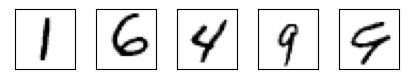
\includegraphics[width=\textwidth]{Images/mnist.png}
\caption[Some examples of the MNIST dataset]{Some examples of the MNIST \cite{mnist} dataset.}
\label{fig:mnist}
\end{figure}

\begin{figure}
\centering
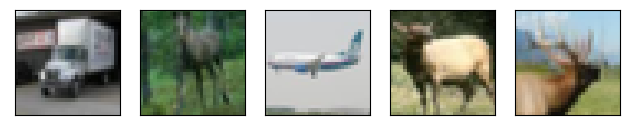
\includegraphics[width=\textwidth]{Images/cifar.png}
\caption[Some examples of the CIFAR-10 dataset]{Some examples of the CIFAR-10 \cite{cifar} dataset.}
\label{fig:cifar}
\end{figure}

\begin{table}
	\centering
	\caption[Model architectures for the MNIST and CIFAR model]{Model architectures for the MNIST and CIFAR models. The architectures are identical to \cite{cw_attack, defensive_distillation}.}
    \begin{tabular}{lll}\toprule
        Layer type     & MNIST Model &CIFAR Model\\ \midrule
		Convolution + \gls{relu}	&$3 \times 3 \times 32$ &$3\times3\times64$\\
		Convolution + \gls{relu}	&$3 \times 3 \times 32$ &$3\times3\times64$\\
		Max Pooling					&$2 \times2$			&$2\times2$\\
		Convolution + \gls{relu}	&$3 \times 3 \times 64$ &$3\times3\times128$\\
		Convolution + \gls{relu}	&$3 \times 3 \times 64$ &$3\times3\times128$\\
		Max Pooling					&$2 \times2$			&$2\times2$\\
		Fully Connected + \gls{relu}&200					&256\\
		Fully Connected + \gls{relu}&200					&256\\
		Softmax						&10						&10\\
        \bottomrule
    \end{tabular}
    \label{tbl:architectures}
\end{table}

The stateful defense mechanism \cite{chen_stateful_2019} will use a query bounded detector buffer of 1000 queries per user. The value of $k$ will be set to 50, as suggested by the authors of the paper. A threshold is determined in order to achieve a 0.1\% false positive detection rate on the training data. The detector buffer will be cleared after each detection to simulate the creation of a new account.\\

The algorithm receives a budget of \num{25000} queries to create an adversarial example. The final adversarial example will be evaluated on the $L_2$-distance to the original image and the total number of detections by the stateful defense mechanism.

\section{Determining the baseline}\label{sec:baseline}
The goal of this subsection is to determine a baseline to which all future algorithms will be compared. The baseline will be a vanilla \gls{bba} using the same hyperparameters as suggested in \cite{brunner_guessing_2019}. The orthogonal step will be set to 0.05 and the source step to 0.002. Both the Perlin noise improvement and the regional masking improvement will be used. No gradients of surrogate models will be calculated as the authors of the paper already mentioned that the improvement was marginal.\\

Table \ref{tbl:baseline} reports the average $L_2$-distance and the average number of detections for the different datasets. 

\begin{table}
	\centering
	\caption[Baseline results]{Results for the \gls{bba} baseline approach on MNIST and CIFAR-10 dataset.}
	\label{tbl:baseline}
	\begin{tabular}{lrrrr}\toprule
			& \multicolumn{2}{c}{MNIST} &\multicolumn{2}{c}{CIFAR} \\ \cmidrule(r){2-3} \cmidrule(r){4-5}
	Attack				&Distance	&Detections	&Distance	&Detections \\ \midrule
	Baseline \gls{bba}	&2.807		&413		&1.306			&474 \\ \bottomrule
	
	\end{tabular}
\end{table}

\section{Applying PSO to BBA} \label{sec:combining_pso_bba}
As mentioned in section \ref{sec:optimization_approach}, previous attempts to craft adversarial example using \gls{pso} used \gls{pso} to guide adversarial examples through the search space closer to the original image. This work aims to combine the benefits of \gls{pso} and an existing decision-based attack such as \gls{bba}.\\

Vanilla \gls{bba} has the disadvantage that, depending on the starting position, it might get trapped in a local optimum. By using \gls{pso} in combination with \gls{bba}, multiple starting positions can be explored and the probability of getting trapped is lowered. The intuition behind this idea is shown in Figure \ref{fig:applying_pso_to_bba}. The more starting positions there are, the higher the probability of finding the global optimum. There is however a clear trade-off in terms of efficiency. By having $n$ different starting positions, the query budget is essentially reduced by a factor~$n$ for each starting position.\\

The efficiency reduction does not have to pose a problem due to the implicit communication in the swarm. Particles can move to promising regions in the search space based on the information of their peers. The promising regions are therefore more queried.\\ 

The proposed \gls{pso}-\gls{bba} algorithm works as follows. Particles will perform a more aggressive version of \gls{bba}. The initial source step~$\epsilon$ is set significantly higher than in the vanilla version. The increased source step might cause the particle to end up in a non-adversarial decision region. Once this happens, the standard \gls{pso} equations (\ref{eq:velocity_update} and \ref{eq:position_update}) are used to guide the particle back to the adversarial region. Later refinements of this algorithms will deal with attack iterations. An attack iteration is defined as a specified budget of the aggressive \gls{bba} (50 queries in all experiments) or a single query submission using the \gls{pso} rules.\\

The inertia weight of the \gls{pso} equations is determined by the linearly decaying scheme of equation \ref{eq:weight}, with the weight decaying from 1 to 0. The acceleration coefficients $c$ are set based on an idea of multi-group \gls{pso}. Two groups with opposite acceleration coefficients are created. This approach helps escape local optima \cite{opposite_cs}. The equations for both $c_p$ and $c_g$ are:

\begin{align*}
c_p &= 
\begin{cases}
	\max(A1, A2), &\text{if } i\bmod 2 = 0\\
	\min(A1, A2), &\text{else}
\end{cases}\\
c_g &=
\begin{cases}
	\min(A1, A2), &\text{if } i\bmod 2 = 0\\
	\max(A1, A2), &\text{else}
\end{cases}\\
\end{align*} 

Here $i$ is the index of the particle in its swarm. The values of $A1$ and $A2$ are 1 and 2 respectively. These values are suggested by the authors of \cite{suryanto2020}.\\

The source step~$\epsilon$ will be changed after every iteration of the attack. Two separate multipliers are used to respectively increase and decrease the value of this parameter. The value of $\epsilon$ is slightly increased if the new position is still adversarial. Likewise it is decreased if the position is no longer adversarial.\\

By using \gls{pso} in combination with \gls{bba}, the advantage of multiple starting points, as explained in Figure \ref{fig:applying_pso_to_bba}, can be exploited, without having a less efficient attack as a whole. Whenever particles end up in non-adversarial regions, they will move closer to the best known position in the swarm due to the \gls{pso} equations. At then end of the attack, most particles will be in the same area of the search space, allowing for more exploitation in this specific area.\\

The \gls{pso} framework requires a fitness function the quantify the fitness of a position for the problem at hand. The authors of AdversarialPSO \cite{mosli2019they} suggested the following fitness function~$f$:

\begin{align}
	f(x) = |p_{x} - p_{x^{\prime}}| - \frac{c}{n}\|x-x^\prime\|_2   \label{eq:old_fitness}
\end{align}

Where $x$ is the position of the particle, $x^\prime$ is the original image, $p_{x}$ and $p_{x^\prime}$ are the confidence scores of the model in predicting the label of $x$ and $x^\prime$ respectively and $c$ is a constant to weight the penalty. However, as discussed in section \ref{sec:threat_model}, the confidence scores are not available for this specific attack. The fitness function in equation \ref{eq:old_fitness} also assumes that the position $x$ will always be adversarial. This will not be the case in the proposed algorithm. The fitness function will therefore be altered to the following:
\begin{align}
	f(x) = 
	\begin{cases}
 		\| x - x^\prime\|_2,	&\text{if } x \text{ is adversarial}\\
 		+\infty, 		& \text{else}
	\end{cases}
\end{align}

The infinite value for the fitness function inside non-adversarial decision regions acts as a penalty, causing the particles to quickly diverge from these regions.\\

The same set of experiments as in section \ref{sec:baseline} has been performed. The experiments have been done using attacks with both five and ten particles. The initial step sizes have been set to 0.25 and 0.20 for MNIST and CIFAR respectively. The values for the increasing and decreasing multiplier have been set to 1.05 and 0.99 for both datasets. The results of the experiments can be found in Table \ref{tbl:pso_bba}.\\

The five particle \gls{pso}-\gls{bba} algorithm outperforms the baseline in terms of distance to the original image on both datasets. This is not the case for the ten particle version. The high number of particles requires sufficient queries in the beginning of the attack in order to discover promising regions in the high dimensional search space of CIFAR. This exploration requires more queries than the query budget allows. The number of detections is lower for all variants of \gls{pso}-\gls{bba}. The different starting points have the added advantage that initial queries are more spread out over the search space. These queries are therefore less similar and the detector will not flag as much attacks. This effect can be seen in Figure \ref{fig:detections_bba_vs_pso_bba} for the MNIST experiments.\\

The number of detections drops as the number of particles increases. This was to be expected from the intuition behind \gls{pso}-\gls{bba}. However, the average $L_2$-distance to the original image is higher for ten particles compared to five. To reduce the number of different parameters in future refinements, only swarms with five particles will be considered from here on.\\ 

\begin{figure}
	\centering
\tikzset{every picture/.style={line width=0.75pt}} %set default line width to 0.75pt        

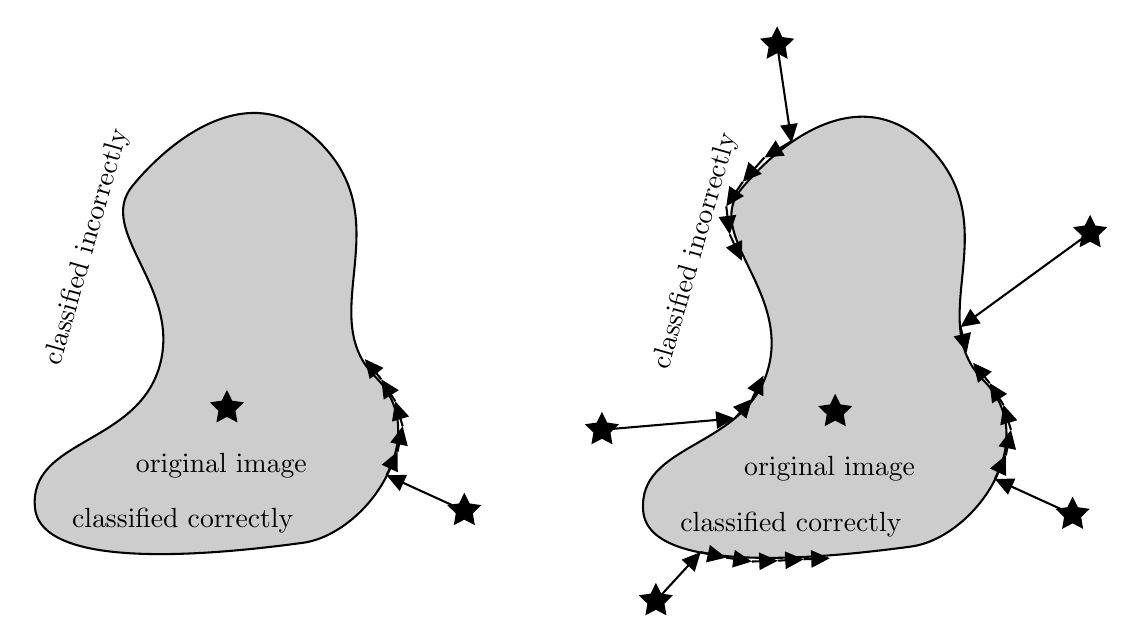
\begin{tikzpicture}[x=0.75pt,y=0.75pt,yscale=-1,xscale=1]
%uncomment if require: \path (0,300); %set diagram left start at 0, and has height of 300

%Shape: Polygon Curved [id:ds39418321723754923] 
\draw  [fill={rgb, 255:red, 155; green, 155; blue, 155 }  ,fill opacity=0.5 ] (365.12,90.5) .. controls (383.12,68.5) and (424.12,34.5) .. (458.12,72.5) .. controls (492.12,110.5) and (453.12,153.5) .. (482.12,182.5) .. controls (511.12,211.5) and (477.12,258.5) .. (447.12,262.5) .. controls (417.12,266.5) and (321.12,278.5) .. (318.12,245.5) .. controls (315.12,212.5) and (367.12,215.5) .. (378.12,177.5) .. controls (389.12,139.5) and (347.12,112.5) .. (365.12,90.5) -- cycle ;
%Shape: Star [id:dp17995230177708343] 
\draw  [fill={rgb, 255:red, 0; green, 0; blue, 0 }  ,fill opacity=1 ] (410.62,190) -- (412.83,194.47) -- (417.76,195.18) -- (414.19,198.66) -- (415.03,203.57) -- (410.62,201.25) -- (406.22,203.57) -- (407.06,198.66) -- (403.49,195.18) -- (408.42,194.47) -- cycle ;
%Shape: Star [id:dp263511542953333] 
\draw  [fill={rgb, 255:red, 0; green, 0; blue, 0 }  ,fill opacity=1 ] (382.62,13) -- (384.83,17.47) -- (389.76,18.18) -- (386.19,21.66) -- (387.03,26.57) -- (382.62,24.25) -- (378.22,26.57) -- (379.06,21.66) -- (375.49,18.18) -- (380.42,17.47) -- cycle ;
%Straight Lines [id:da12241666866362477] 
\draw    (382.62,20.5) -- (389.19,64.95) ;
\draw [shift={(389.62,67.92)}, rotate = 261.6] [fill={rgb, 255:red, 0; green, 0; blue, 0 }  ][line width=0.08]  [draw opacity=0] (8.93,-4.29) -- (0,0) -- (8.93,4.29) -- cycle    ;
%Straight Lines [id:da7985170559413728] 
\draw    (389.79,67.08) -- (379.03,73.54) ;
\draw [shift={(376.46,75.08)}, rotate = 329.04] [fill={rgb, 255:red, 0; green, 0; blue, 0 }  ][line width=0.08]  [draw opacity=0] (8.93,-4.29) -- (0,0) -- (8.93,4.29) -- cycle    ;
%Straight Lines [id:da5286207592270582] 
\draw    (376.46,75.08) -- (368.11,84.5) ;
\draw [shift={(366.12,86.75)}, rotate = 311.53] [fill={rgb, 255:red, 0; green, 0; blue, 0 }  ][line width=0.08]  [draw opacity=0] (8.93,-4.29) -- (0,0) -- (8.93,4.29) -- cycle    ;
%Straight Lines [id:da4098354744836743] 
\draw    (366.12,86.75) -- (359.8,96.1) ;
\draw [shift={(358.12,98.58)}, rotate = 304.06] [fill={rgb, 255:red, 0; green, 0; blue, 0 }  ][line width=0.08]  [draw opacity=0] (8.93,-4.29) -- (0,0) -- (8.93,4.29) -- cycle    ;
%Straight Lines [id:da7402027038712158] 
\draw    (358.12,98.58) -- (359.42,109.11) ;
\draw [shift={(359.79,112.08)}, rotate = 262.96] [fill={rgb, 255:red, 0; green, 0; blue, 0 }  ][line width=0.08]  [draw opacity=0] (8.93,-4.29) -- (0,0) -- (8.93,4.29) -- cycle    ;
%Straight Lines [id:da22742294505428506] 
\draw    (359.79,112.08) -- (364.37,122.03) ;
\draw [shift={(365.62,124.75)}, rotate = 245.27] [fill={rgb, 255:red, 0; green, 0; blue, 0 }  ][line width=0.08]  [draw opacity=0] (8.93,-4.29) -- (0,0) -- (8.93,4.29) -- cycle    ;
%Shape: Boxed Line [id:dp17555971988752717] 
\draw    (362.2,200.74) -- (368.55,193.64) ;
\draw [shift={(370.55,191.4)}, rotate = 131.8] [fill={rgb, 255:red, 0; green, 0; blue, 0 }  ][line width=0.08]  [draw opacity=0] (8.93,-4.29) -- (0,0) -- (8.93,4.29) -- cycle    ;
%Shape: Star [id:dp5469311004467188] 
\draw  [fill={rgb, 255:red, 0; green, 0; blue, 0 }  ,fill opacity=1 ] (533.42,103.8) -- (535.63,108.27) -- (540.56,108.98) -- (536.99,112.46) -- (537.83,117.37) -- (533.42,115.05) -- (529.02,117.37) -- (529.86,112.46) -- (526.29,108.98) -- (531.22,108.27) -- cycle ;
%Shape: Star [id:dp8199494411723183] 
\draw  [fill={rgb, 255:red, 0; green, 0; blue, 0 }  ,fill opacity=1 ] (525,239.51) -- (527.2,243.97) -- (532.13,244.69) -- (528.57,248.17) -- (529.41,253.07) -- (525,250.76) -- (520.59,253.07) -- (521.43,248.17) -- (517.87,244.69) -- (522.8,243.97) -- cycle ;
%Shape: Star [id:dp3621439940158031] 
\draw  [fill={rgb, 255:red, 0; green, 0; blue, 0 }  ,fill opacity=1 ] (324.22,281.14) -- (326.43,285.61) -- (331.36,286.32) -- (327.79,289.8) -- (328.63,294.71) -- (324.22,292.39) -- (319.82,294.71) -- (320.66,289.8) -- (317.09,286.32) -- (322.02,285.61) -- cycle ;
%Shape: Star [id:dp886425904787334] 
\draw  [fill={rgb, 255:red, 0; green, 0; blue, 0 }  ,fill opacity=1 ] (298.22,198.74) -- (300.43,203.21) -- (305.36,203.92) -- (301.79,207.4) -- (302.63,212.31) -- (298.22,209.99) -- (293.82,212.31) -- (294.66,207.4) -- (291.09,203.92) -- (296.02,203.21) -- cycle ;
%Straight Lines [id:da29737150039250193] 
\draw    (533.42,111.3) -- (473.43,154.98) ;
\draw [shift={(471,156.74)}, rotate = 323.95] [fill={rgb, 255:red, 0; green, 0; blue, 0 }  ][line width=0.08]  [draw opacity=0] (8.93,-4.29) -- (0,0) -- (8.93,4.29) -- cycle    ;
%Straight Lines [id:da564242749820822] 
\draw    (298.22,206.24) -- (359.21,201) ;
\draw [shift={(362.2,200.74)}, rotate = 175.09] [fill={rgb, 255:red, 0; green, 0; blue, 0 }  ][line width=0.08]  [draw opacity=0] (8.93,-4.29) -- (0,0) -- (8.93,4.29) -- cycle    ;
%Straight Lines [id:da8824188996602935] 
\draw    (525,247.01) -- (490.26,231.18) ;
\draw [shift={(487.53,229.94)}, rotate = 24.49] [fill={rgb, 255:red, 0; green, 0; blue, 0 }  ][line width=0.08]  [draw opacity=0] (8.93,-4.29) -- (0,0) -- (8.93,4.29) -- cycle    ;
%Straight Lines [id:da172043009485096] 
\draw    (324.22,288.64) -- (343.77,267.35) ;
\draw [shift={(345.8,265.14)}, rotate = 132.55] [fill={rgb, 255:red, 0; green, 0; blue, 0 }  ][line width=0.08]  [draw opacity=0] (8.93,-4.29) -- (0,0) -- (8.93,4.29) -- cycle    ;
%Shape: Boxed Line [id:dp5913488094519332] 
\draw    (370.55,191.4) -- (374.75,182.84) ;
\draw [shift={(376.07,180.15)}, rotate = 116.11] [fill={rgb, 255:red, 0; green, 0; blue, 0 }  ][line width=0.08]  [draw opacity=0] (8.93,-4.29) -- (0,0) -- (8.93,4.29) -- cycle    ;
%Shape: Boxed Line [id:dp8616221435272089] 
\draw    (487.53,229.94) -- (491.55,221.3) ;
\draw [shift={(492.81,218.58)}, rotate = 114.93] [fill={rgb, 255:red, 0; green, 0; blue, 0 }  ][line width=0.08]  [draw opacity=0] (8.93,-4.29) -- (0,0) -- (8.93,4.29) -- cycle    ;
%Shape: Boxed Line [id:dp5796326247856174] 
\draw    (492.81,218.58) -- (494.7,209.24) ;
\draw [shift={(495.29,206.29)}, rotate = 101.39] [fill={rgb, 255:red, 0; green, 0; blue, 0 }  ][line width=0.08]  [draw opacity=0] (8.93,-4.29) -- (0,0) -- (8.93,4.29) -- cycle    ;
%Shape: Boxed Line [id:dp044334919963415986] 
\draw    (495.29,206.29) -- (492.57,197.16) ;
\draw [shift={(491.71,194.29)}, rotate = 73.42] [fill={rgb, 255:red, 0; green, 0; blue, 0 }  ][line width=0.08]  [draw opacity=0] (8.93,-4.29) -- (0,0) -- (8.93,4.29) -- cycle    ;
%Shape: Boxed Line [id:dp4387546700476397] 
\draw    (491.71,194.29) -- (486.61,186.24) ;
\draw [shift={(485,183.71)}, rotate = 57.58] [fill={rgb, 255:red, 0; green, 0; blue, 0 }  ][line width=0.08]  [draw opacity=0] (8.93,-4.29) -- (0,0) -- (8.93,4.29) -- cycle    ;
%Shape: Boxed Line [id:dp8947094222533136] 
\draw    (485,183.71) -- (478.98,176.32) ;
\draw [shift={(477.09,173.99)}, rotate = 50.85] [fill={rgb, 255:red, 0; green, 0; blue, 0 }  ][line width=0.08]  [draw opacity=0] (8.93,-4.29) -- (0,0) -- (8.93,4.29) -- cycle    ;
%Shape: Boxed Line [id:dp8126738394252795] 
\draw    (471,156.74) -- (473.27,166) ;
\draw [shift={(473.99,168.91)}, rotate = 256.19] [fill={rgb, 255:red, 0; green, 0; blue, 0 }  ][line width=0.08]  [draw opacity=0] (8.93,-4.29) -- (0,0) -- (8.93,4.29) -- cycle    ;
%Shape: Boxed Line [id:dp14754319972001273] 
\draw    (345.8,265.14) -- (355.11,267.18) ;
\draw [shift={(358.04,267.82)}, rotate = 192.33] [fill={rgb, 255:red, 0; green, 0; blue, 0 }  ][line width=0.08]  [draw opacity=0] (8.93,-4.29) -- (0,0) -- (8.93,4.29) -- cycle    ;
%Shape: Boxed Line [id:dp8374639915608668] 
\draw    (358.04,267.82) -- (367.46,269.26) ;
\draw [shift={(370.43,269.71)}, rotate = 188.71] [fill={rgb, 255:red, 0; green, 0; blue, 0 }  ][line width=0.08]  [draw opacity=0] (8.93,-4.29) -- (0,0) -- (8.93,4.29) -- cycle    ;
%Shape: Boxed Line [id:dp496623104677657] 
\draw    (370.43,269.71) -- (379.95,269.39) ;
\draw [shift={(382.95,269.29)}, rotate = 178.04] [fill={rgb, 255:red, 0; green, 0; blue, 0 }  ][line width=0.08]  [draw opacity=0] (8.93,-4.29) -- (0,0) -- (8.93,4.29) -- cycle    ;
%Shape: Boxed Line [id:dp34473561543285314] 
\draw    (382.95,269.29) -- (392.47,268.77) ;
\draw [shift={(395.46,268.61)}, rotate = 176.92] [fill={rgb, 255:red, 0; green, 0; blue, 0 }  ][line width=0.08]  [draw opacity=0] (8.93,-4.29) -- (0,0) -- (8.93,4.29) -- cycle    ;
%Shape: Boxed Line [id:dp22829712791209555] 
\draw    (395.46,268.61) -- (404.98,268.23) ;
\draw [shift={(407.98,268.11)}, rotate = 177.71] [fill={rgb, 255:red, 0; green, 0; blue, 0 }  ][line width=0.08]  [draw opacity=0] (8.93,-4.29) -- (0,0) -- (8.93,4.29) -- cycle    ;

%Shape: Polygon Curved [id:ds013419098702227128] 
\draw  [fill={rgb, 255:red, 155; green, 155; blue, 155 }  ,fill opacity=0.5 ] (72.05,88.7) .. controls (90.05,66.7) and (131.05,32.7) .. (165.05,70.7) .. controls (199.05,108.7) and (160.05,151.7) .. (189.05,180.7) .. controls (218.05,209.7) and (184.05,256.7) .. (154.05,260.7) .. controls (124.05,264.7) and (28.05,276.7) .. (25.05,243.7) .. controls (22.05,210.7) and (74.05,213.7) .. (85.05,175.7) .. controls (96.05,137.7) and (54.05,110.7) .. (72.05,88.7) -- cycle ;
%Shape: Star [id:dp9534459695500062] 
\draw  [fill={rgb, 255:red, 0; green, 0; blue, 0 }  ,fill opacity=1 ] (117.55,188.2) -- (119.76,192.67) -- (124.68,193.38) -- (121.12,196.86) -- (121.96,201.77) -- (117.55,199.45) -- (113.14,201.77) -- (113.99,196.86) -- (110.42,193.38) -- (115.35,192.67) -- cycle ;
%Shape: Star [id:dp3150974101447812] 
\draw  [fill={rgb, 255:red, 0; green, 0; blue, 0 }  ,fill opacity=1 ] (231.93,237.71) -- (234.13,242.17) -- (239.06,242.89) -- (235.49,246.37) -- (236.34,251.28) -- (231.93,248.96) -- (227.52,251.28) -- (228.36,246.37) -- (224.79,242.89) -- (229.72,242.17) -- cycle ;
%Straight Lines [id:da8721626382201679] 
\draw    (231.93,245.21) -- (197.19,229.38) ;
\draw [shift={(194.46,228.14)}, rotate = 24.49] [fill={rgb, 255:red, 0; green, 0; blue, 0 }  ][line width=0.08]  [draw opacity=0] (8.93,-4.29) -- (0,0) -- (8.93,4.29) -- cycle    ;
%Shape: Boxed Line [id:dp35233924811215767] 
\draw    (194.46,228.14) -- (198.48,219.5) ;
\draw [shift={(199.74,216.78)}, rotate = 114.93] [fill={rgb, 255:red, 0; green, 0; blue, 0 }  ][line width=0.08]  [draw opacity=0] (8.93,-4.29) -- (0,0) -- (8.93,4.29) -- cycle    ;
%Shape: Boxed Line [id:dp47377705399021885] 
\draw    (199.74,216.78) -- (201.62,207.44) ;
\draw [shift={(202.22,204.5)}, rotate = 101.39] [fill={rgb, 255:red, 0; green, 0; blue, 0 }  ][line width=0.08]  [draw opacity=0] (8.93,-4.29) -- (0,0) -- (8.93,4.29) -- cycle    ;
%Shape: Boxed Line [id:dp01327277725498055] 
\draw    (202.22,204.5) -- (199.5,195.36) ;
\draw [shift={(198.64,192.49)}, rotate = 73.42] [fill={rgb, 255:red, 0; green, 0; blue, 0 }  ][line width=0.08]  [draw opacity=0] (8.93,-4.29) -- (0,0) -- (8.93,4.29) -- cycle    ;
%Shape: Boxed Line [id:dp6860848467619505] 
\draw    (198.64,192.49) -- (193.53,184.44) ;
\draw [shift={(191.92,181.91)}, rotate = 57.58] [fill={rgb, 255:red, 0; green, 0; blue, 0 }  ][line width=0.08]  [draw opacity=0] (8.93,-4.29) -- (0,0) -- (8.93,4.29) -- cycle    ;
%Shape: Boxed Line [id:dp2849658598230065] 
\draw    (191.92,181.91) -- (185.91,174.52) ;
\draw [shift={(184.01,172.19)}, rotate = 50.85] [fill={rgb, 255:red, 0; green, 0; blue, 0 }  ][line width=0.08]  [draw opacity=0] (8.93,-4.29) -- (0,0) -- (8.93,4.29) -- cycle    ;


% Text Node
\draw (107.14,250.13) node   [align=left] {\begin{minipage}[lt]{96.27pt}\setlength\topsep{0pt}
classified correctly
\end{minipage}};
% Text Node
\draw (51.61,113.14) node  [rotate=-286.01] [align=left] {\begin{minipage}[lt]{96.27pt}\setlength\topsep{0pt}
classified incorrectly
\end{minipage}};
% Text Node
\draw (119.05,223.33) node   [align=left] {\begin{minipage}[lt]{68pt}\setlength\topsep{0pt}
original image
\end{minipage}};
% Text Node
\draw (400.21,251.93) node   [align=left] {\begin{minipage}[lt]{96.27pt}\setlength\topsep{0pt}
classified correctly
\end{minipage}};
% Text Node
\draw (344.71,114.94) node  [rotate=-286.01] [align=left] {\begin{minipage}[lt]{96.27pt}\setlength\topsep{0pt}
classified incorrectly
\end{minipage}};
% Text Node
\draw (412.12,225.13) node   [align=left] {\begin{minipage}[lt]{68pt}\setlength\topsep{0pt}
original image
\end{minipage}};


\end{tikzpicture}	
\caption[Intuition of multiple starting points]{The vanilla version of \gls{bba} might get stuck in a local optimum depending on the starting point (left plot). By starting from multiple positions, the probability that \gls{bba} gets stuck in a local optimum is reduced (right plot). The multiple starting points are particles in a \gls{pso} swarm. Image inspired by \cite{boundary_attack}.}
\label{fig:applying_pso_to_bba}
\end{figure}

\begin{figure}
\centering
\begin{tikzpicture}
\begin{axis}[width=12cm, height=5cm, xmin=0,xmax=25000, xlabel=Calls, ylabel=Detections, tick label style={/pgf/number format/fixed}, scaled ticks=false, enlarge x limits=0.01, xtick={0,5000,10000,15000,20000,25000},legend pos=north west,	legend style={draw=none},]
\addplot table[blue,col sep=comma,x index=1,y expr=\thisrowno{0},mark=none] {Data/detections_bba_mnist.csv};
\addlegendentry{\gls{bba}};
\addplot table[color=red,col sep=comma,x index=1,y expr=\thisrowno{0},mark=none] {Data/detections_bba_pso_mnist.csv};
\addlegendentry{\gls{pso}-\gls{bba}};

\addplot [name path=lower_bba, fill=none, draw=none] table [
    x index=1, y expr=\thisrowno{0} - \thisrow{ci},col sep=comma]{Data/detections_bba_mnist.csv};
\addplot [name path=upper_bba, fill=none, draw=none] table [
    x index=1, y expr=\thisrowno{0} + \thisrow{ci},col sep=comma]{Data/detections_bba_mnist.csv};
\addplot[blue!60, fill opacity=0.2] fill between[of=lower_bba and upper_bba];


\addplot [name path=lower_pso, fill=none, draw=none] table [
    x index=1, y expr=\thisrowno{0} - \thisrow{ci},col sep=comma]{Data/detections_bba_pso_mnist.csv};
\addplot [name path=upper_pso, fill=none, draw=none] table [
    x index=1, y expr=\thisrowno{0} + \thisrow{ci},col sep=comma]{Data/detections_bba_pso_mnist.csv};
\addplot[red!60, fill opacity=0.2] fill between[of=lower_pso and upper_pso];


\end{axis}
\end{tikzpicture}
\caption[Detections of the different attacks]{The cumulative number of detections for different attack algorithms for the MNIST experiments. The number of detections of the \gls{bba} algorithm steadily increases with the number of calls. The number of detections of the \gls{pso}-\gls{bba} algorithm increases more slowly in the beginning due to the dispersed nature of the attack. The increase is more sharp near the end of the attack when the particles converge. The plot shows the 95\% confidence regions around the graphs.}
\label{fig:detections_bba_vs_pso_bba}
\end{figure}

\begin{table}
	\centering
	\caption[PSO-BBA results]{Results for the \gls{pso}-\gls{bba} approach on MNIST and CIFAR-10 dataset.}
	\label{tbl:pso_bba}
	\begin{tabular}{lrrrr}\toprule
			& \multicolumn{2}{c}{MNIST} &\multicolumn{2}{c}{CIFAR} \\ \cmidrule(r){2-3} \cmidrule(r){4-5}
	Attack				&Distance	&Detections	&Distance	&Detections \\ \midrule
	Baseline \gls{bba}	&2.807		&413		&1.306			&474 \\
	\gls{pso}-\gls{bba} (5 particles)	&2.712			&138			&1.239				&257 \\ 
	\gls{pso}-\gls{bba} (10 particles)	&3.157			&44			&2.290				&184 \\
	
	\bottomrule
	
	\end{tabular}
\end{table}

\section{Towards distribution of the attack}
The stateful defense mechanism \cite{chen_stateful_2019} makes the assumption that there is no collaboration between adversaries. Based on this assumption, each account or user will have its own detector buffer. This subsection aims to exploit this assumption by distributing the query submission over multiple accounts.\\

By distributing the query submissions over multiple accounts, the number of total detection should be reduced compared to \gls{bba} due to two reasons. The first reason is obvious. If a budget of \num{25000} queries is distributed over $N$ accounts, then every account will submit \num{25000} / $N$ queries. The less queries there are submitted, the less potential attacks will be detected. The second reason is due to \gls{pso}. As stated before, the different particles reside in different parts of the search space. This means that a detector buffer of a specific account will contain queries from all over the search space, causing the inter query distances to be larger. The latter reason was also present in the algorithm described in section \ref{sec:combining_pso_bba}.\\

It should be noted that there is only distribution at the query submission level. The algorithm itself will be executed on one machine without the need for distribution. Even the query submission can be done from one machine by constantly changing the \gls{api} key or by logging in and out of a specific account whenever it is needed. This approach makes the assumption that the \gls{api} under attack does not track the IP~address of the machine that submitted the query. Multiple machines might therefore be more convenient in a real attack setting.\\

This work simulates the multiple machines setting by having separate node (or machine) objects on the same machine. Instead of having a detector buffer for each node at the location of the model, the responsibility is moved upstream to the nodes themselves. Each node will have a buffer to which the query will be added. All queries will be passed to the model afterwards. In Figure \ref{fig:distribution_overview}, the distribution is shown schematically.\\

The queries will be distributed over the nodes based on a distribution scheme. Three different distribution schemes will be used in the experiments. The first two schemes are inspired by the \gls{rr} scheduling algorithm \cite{round_robin} and will be called the \gls{rr} and \gls{mrr} distribution schemes. The third distribution scheme will be built on the assumption that the inter query distance in the detector buffers needs to be maximized.\\

The \gls{rr} distribution scheme is fairly straightforward. The outgoing queries of the algorithm will be evenly distributed over the nodes in circular order. This scheme does not have a notion of the underlying attack. This can cause successive queries forwarded to the same node to be relatively close together by chance.\\  

The \gls{mrr} distribution scheme maps a particle to a node for the entire duration of an attack iteration. The queries submitted by a single particle during one attack iteration are relatively close together, but this approach ensures that all particles will submit queries to all nodes. This might ultimately cause less detections. The \gls{mrr} distribution scheme maps a number of particles on a number of nodes. If the amount of particles is equal to the number of nodes then the mapping is straightforward. If the number of nodes is less than the number of particles then dummy nodes are introduced in the mapping. The dummy nodes forward their received queries to a random existing node. The random node changes every rotation. If the number of particles is less than the number of nodes then dummy particles that do not submit queries, are introduced. After every attack iteration, the mapping rotates. The mapping process is shown in Figure \ref{fig:round_robin}.\\ 

The ultimate goal of the attack is to evade the stateful detection mechanism that defends the model under attack. Potential attacks are flagged based on the inter query distance in a detector buffer. The distance-based distribution scheme tries to exploit the defense. Instead of distributing queries over nodes in a \gls{rr}-fashion, queries are submitted to nodes based on the distance to the previously submitted queries to this node. The node with the highest average distance to the previously submitted queries is selected. For this purpose, every node will hold an internal buffer of queries. The size of this buffer can be chosen by the attacker, as can the distance metric. Standard $L_2$-distance can be chosen, but this has the same pitfalls as discussed in section \ref{sec:stateful_detection}. It is also possible to train another similarity encoder and use the $L_2$-distance in the embedded space in order to resemble the defense more closely. The distribution schemes will be called \gls{db} and \gls{edb} distribution schemes respectively.\\

The experiments performed in this section will use a buffer size at each node of 20 for both the \gls{db} and \gls{edb} distribution schemes. The similarity encoder in the case of the \gls{edb} scheme will be trained on the test data of the respective dataset and has an output dimension of 128. The results of the experiments can be found in Table \ref{tbl:d_pso_bba}.\\



\begin{figure}
\centering
\begin{tikzpicture}
\begin{scope}[every node/.style={rectangle,thick,draw,anchor=base, minimum width=20mm}]
	\node[align=center] (N1) at (3,5) {Node 1};
	\node[align=center] (N2) at (3,4) {Node 2};
	\node[align=center] (N3) at (3,3) {Node 3};
	\node[align=center] (NN) at (3,1) {Node $N$};
\end{scope}

\node[align=center,anchor=base, minimum width=20mm,rectangle] (N) at (3,2) {$\ldots$};

\begin{scope}[every node/.style={rectangle,thick,draw,anchor=base,minimum width=20mm, minimum height=10mm}]
	\node[align=right, left= 35mm of N3] (A) {Algorithm};
	\node[align=left, right= 35mm of N3] (M) {Model};
\end{scope}

\begin{scope}[]
	\path [->] (A.east) edge (N1.west);
	\path [->] (A.east) edge (N2.west);
	\path [->] (A.east) edge (N3.west);
%	\path [->] (A.east) edge (N.west);
	\path [->] (A.east) edge (NN.west);

	\path [->] (N1.east) edge (M.west);
	\path [->] (N2.east) edge (M.west);
	\path [->] (N3.east) edge (M.west);
%	\path [->] (N.east) edge (M.west);
	\path [->] (NN.east) edge (M.west);	
\end{scope}
\end{tikzpicture}
\caption[Schematic overview of the query submission distribution]{Schematic overview of the query submission distribution. Each arrow represents a query. The algorithm distributes the queries over the different nodes. Every node forwards its received queries to the model using the corresponding account. In a real setting, the model will have a detector buffer for every account. In this work the buffers are located on the nodes themselves.}
\label{fig:distribution_overview}
\end{figure}

\begin{table}
	\centering
	\caption[Distributed PSO-BBA results]{Results for the distributed \gls{pso}-\gls{bba} approaches on MNIST and CIFAR-10 dataset.}
	\label{tbl:d_pso_bba}
	\begin{tabular}{lrrrr}\toprule
			& \multicolumn{2}{c}{MNIST} &\multicolumn{2}{c}{CIFAR} \\ \cmidrule(r){2-3} \cmidrule(r){4-5}
	Attack				&Distance	&Detections	&Distance	&Detections \\ \midrule
	Baseline \gls{bba}							&2.807	&413	&1.306	&474 \\
	\gls{pso}-\gls{bba} 						&2.712	&138	&1.329	&257 \\ \addlinespace[\linespace] 
	\gls{rr}-\gls{pso}-\gls{bba} (5 nodes) 		&2.712	&124	&1.239	&224 \\
	\gls{rr}-\gls{pso}-\gls{bba} (10 nodes) 	&2.712	&104	&1.239	&202 \\	\addlinespace[\linespace]
	\gls{mrr}-\gls{pso}-\gls{bba} (5 nodes)		&2.712	&110	&1.239	&227 \\
	\gls{mrr}-\gls{pso}-\gls{bba} (10 nodes)	&2.712	&93		&1.239	&206 \\ \addlinespace[\linespace]
	\gls{db}-\gls{pso}-\gls{bba} (5 nodes)		&2.712	&107	&1.239	&230 \\
	\gls{db}-\gls{pso}-\gls{bba} (10 nodes)		&2.712	&87		&1.239	&207 \\ \addlinespace[\linespace]
	\gls{edb}-\gls{pso}-\gls{bba} (5 nodes)		&2.712	&108	&1.239	&229 \\
	\gls{edb}-\gls{pso}-\gls{bba} (10 nodes)	&2.712	&88		&1.239	&205 \\
	\bottomrule
	\end{tabular}
\end{table}

\begin{figure}
\centering
\tikzset{every picture/.style={line width=0.75pt}} %set default line width to 0.75pt        

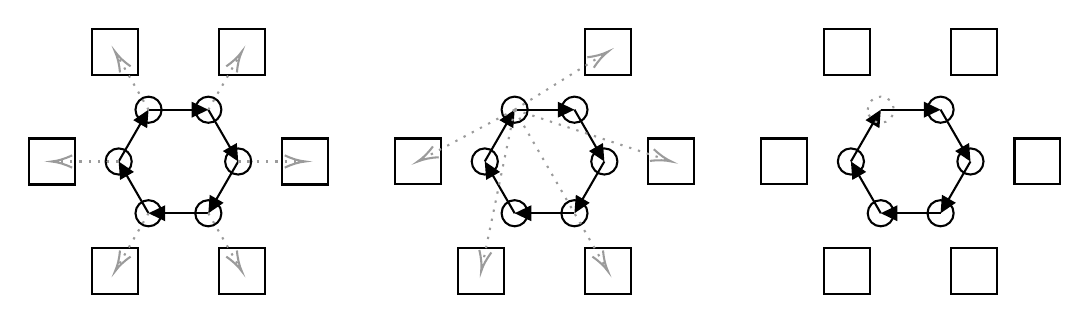
\begin{tikzpicture}[x=0.75pt,y=0.75pt,yscale=-.9,xscale=0.9]
%uncomment if require: \path (0,300); %set diagram left start at 0, and has height of 300

%Shape: Regular Polygon [id:dp6311837881944131] 
\draw  [draw opacity=0] (164.04,130.38) -- (130.11,189.14) -- (62.26,189.14) -- (28.33,130.38) -- (62.26,71.61) -- (130.11,71.61) -- cycle ;
%Shape: Regular Polygon [id:dp734210614935138] 
\draw  [draw opacity=0] (128.18,130.38) -- (112.18,158.09) -- (80.18,158.09) -- (64.18,130.38) -- (80.18,102.67) -- (112.18,102.67) -- cycle ;
%Shape: Circle [id:dp20420366237563004] 
\draw   (121.18,130.38) .. controls (121.18,126.51) and (124.32,123.38) .. (128.18,123.38) .. controls (132.05,123.38) and (135.18,126.51) .. (135.18,130.38) .. controls (135.18,134.24) and (132.05,137.38) .. (128.18,137.38) .. controls (124.32,137.38) and (121.18,134.24) .. (121.18,130.38) -- cycle ;
%Shape: Circle [id:dp5667720968503112] 
\draw   (105.18,158.09) .. controls (105.18,154.22) and (108.32,151.09) .. (112.18,151.09) .. controls (116.05,151.09) and (119.18,154.22) .. (119.18,158.09) .. controls (119.18,161.96) and (116.05,165.09) .. (112.18,165.09) .. controls (108.32,165.09) and (105.18,161.96) .. (105.18,158.09) -- cycle ;
%Shape: Circle [id:dp09001615776819638] 
\draw   (105.18,102.67) .. controls (105.18,98.8) and (108.32,95.67) .. (112.18,95.67) .. controls (116.05,95.67) and (119.18,98.8) .. (119.18,102.67) .. controls (119.18,106.53) and (116.05,109.67) .. (112.18,109.67) .. controls (108.32,109.67) and (105.18,106.53) .. (105.18,102.67) -- cycle ;
%Shape: Circle [id:dp25267892030876826] 
\draw   (73.18,102.67) .. controls (73.18,98.8) and (76.32,95.67) .. (80.18,95.67) .. controls (84.05,95.67) and (87.18,98.8) .. (87.18,102.67) .. controls (87.18,106.53) and (84.05,109.67) .. (80.18,109.67) .. controls (76.32,109.67) and (73.18,106.53) .. (73.18,102.67) -- cycle ;
%Shape: Circle [id:dp9011095802276641] 
\draw   (57.18,130.38) .. controls (57.18,126.51) and (60.32,123.38) .. (64.18,123.38) .. controls (68.05,123.38) and (71.18,126.51) .. (71.18,130.38) .. controls (71.18,134.24) and (68.05,137.38) .. (64.18,137.38) .. controls (60.32,137.38) and (57.18,134.24) .. (57.18,130.38) -- cycle ;
%Shape: Circle [id:dp9002579789917513] 
\draw   (73.18,158.09) .. controls (73.18,154.22) and (76.32,151.09) .. (80.18,151.09) .. controls (84.05,151.09) and (87.18,154.22) .. (87.18,158.09) .. controls (87.18,161.96) and (84.05,165.09) .. (80.18,165.09) .. controls (76.32,165.09) and (73.18,161.96) .. (73.18,158.09) -- cycle ;
%Straight Lines [id:da5872531499507816] 
\draw    (64.18,130.38) -- (78.68,105.26) ;
\draw [shift={(80.18,102.67)}, rotate = 120] [fill={rgb, 255:red, 0; green, 0; blue, 0 }  ][line width=0.08]  [draw opacity=0] (8.93,-4.29) -- (0,0) -- (8.93,4.29) -- cycle    ;
%Straight Lines [id:da6168359296990422] 
\draw    (80.18,102.67) -- (109.18,102.67) ;
\draw [shift={(112.18,102.67)}, rotate = 180] [fill={rgb, 255:red, 0; green, 0; blue, 0 }  ][line width=0.08]  [draw opacity=0] (8.93,-4.29) -- (0,0) -- (8.93,4.29) -- cycle    ;
%Straight Lines [id:da13846207252243437] 
\draw    (112.18,102.67) -- (126.68,127.78) ;
\draw [shift={(128.18,130.38)}, rotate = 240] [fill={rgb, 255:red, 0; green, 0; blue, 0 }  ][line width=0.08]  [draw opacity=0] (8.93,-4.29) -- (0,0) -- (8.93,4.29) -- cycle    ;
%Straight Lines [id:da15864835171123404] 
\draw    (128.18,130.38) -- (113.68,155.49) ;
\draw [shift={(112.18,158.09)}, rotate = 300] [fill={rgb, 255:red, 0; green, 0; blue, 0 }  ][line width=0.08]  [draw opacity=0] (8.93,-4.29) -- (0,0) -- (8.93,4.29) -- cycle    ;
%Straight Lines [id:da1570240528041873] 
\draw    (80.18,158.09) -- (65.68,132.98) ;
\draw [shift={(64.18,130.38)}, rotate = 60] [fill={rgb, 255:red, 0; green, 0; blue, 0 }  ][line width=0.08]  [draw opacity=0] (8.93,-4.29) -- (0,0) -- (8.93,4.29) -- cycle    ;
%Straight Lines [id:da6269615457025413] 
\draw    (112.18,158.09) -- (83.18,158.09) ;
\draw [shift={(80.18,158.09)}, rotate = 360] [fill={rgb, 255:red, 0; green, 0; blue, 0 }  ][line width=0.08]  [draw opacity=0] (8.93,-4.29) -- (0,0) -- (8.93,4.29) -- cycle    ;
%Shape: Square [id:dp8251388573322678] 
\draw   (117.81,176.84) -- (142.41,176.84) -- (142.41,201.44) -- (117.81,201.44) -- cycle ;
%Shape: Square [id:dp205181392666675] 
\draw   (151.74,118.08) -- (176.34,118.08) -- (176.34,142.68) -- (151.74,142.68) -- cycle ;
%Shape: Square [id:dp29815936075322313] 
\draw   (117.81,59.31) -- (142.41,59.31) -- (142.41,83.91) -- (117.81,83.91) -- cycle ;
%Shape: Square [id:dp841488455537714] 
\draw   (49.96,59.31) -- (74.56,59.31) -- (74.56,83.91) -- (49.96,83.91) -- cycle ;
%Shape: Square [id:dp800192330604856] 
\draw   (16.03,118.08) -- (40.63,118.08) -- (40.63,142.68) -- (16.03,142.68) -- cycle ;
%Shape: Square [id:dp672047962326588] 
\draw   (49.96,176.84) -- (74.56,176.84) -- (74.56,201.44) -- (49.96,201.44) -- cycle ;
%Shape: Regular Polygon [id:dp4663627978496028] 
\draw  [draw opacity=0] (360.04,130.37) -- (326.11,189.13) -- (258.26,189.13) -- (224.33,130.37) -- (258.26,71.6) -- (326.11,71.6) -- cycle ;
%Shape: Regular Polygon [id:dp8460846766666963] 
\draw  [draw opacity=0] (324.18,130.37) -- (308.18,158.08) -- (276.18,158.08) -- (260.18,130.37) -- (276.18,102.65) -- (308.18,102.65) -- cycle ;
%Shape: Circle [id:dp28465961252669714] 
\draw   (317.18,130.37) .. controls (317.18,126.5) and (320.32,123.37) .. (324.18,123.37) .. controls (328.05,123.37) and (331.18,126.5) .. (331.18,130.37) .. controls (331.18,134.23) and (328.05,137.37) .. (324.18,137.37) .. controls (320.32,137.37) and (317.18,134.23) .. (317.18,130.37) -- cycle ;
%Shape: Circle [id:dp6382563352290074] 
\draw   (301.18,158.08) .. controls (301.18,154.21) and (304.32,151.08) .. (308.18,151.08) .. controls (312.05,151.08) and (315.18,154.21) .. (315.18,158.08) .. controls (315.18,161.94) and (312.05,165.08) .. (308.18,165.08) .. controls (304.32,165.08) and (301.18,161.94) .. (301.18,158.08) -- cycle ;
%Shape: Circle [id:dp3512284393979799] 
\draw   (301.18,102.65) .. controls (301.18,98.79) and (304.32,95.65) .. (308.18,95.65) .. controls (312.05,95.65) and (315.18,98.79) .. (315.18,102.65) .. controls (315.18,106.52) and (312.05,109.65) .. (308.18,109.65) .. controls (304.32,109.65) and (301.18,106.52) .. (301.18,102.65) -- cycle ;
%Shape: Circle [id:dp887478959629223] 
\draw   (269.18,102.65) .. controls (269.18,98.79) and (272.32,95.65) .. (276.18,95.65) .. controls (280.05,95.65) and (283.18,98.79) .. (283.18,102.65) .. controls (283.18,106.52) and (280.05,109.65) .. (276.18,109.65) .. controls (272.32,109.65) and (269.18,106.52) .. (269.18,102.65) -- cycle ;
%Shape: Circle [id:dp4353947442388322] 
\draw   (253.18,130.37) .. controls (253.18,126.5) and (256.32,123.37) .. (260.18,123.37) .. controls (264.05,123.37) and (267.18,126.5) .. (267.18,130.37) .. controls (267.18,134.23) and (264.05,137.37) .. (260.18,137.37) .. controls (256.32,137.37) and (253.18,134.23) .. (253.18,130.37) -- cycle ;
%Shape: Circle [id:dp7666259147336745] 
\draw   (269.18,158.08) .. controls (269.18,154.21) and (272.32,151.08) .. (276.18,151.08) .. controls (280.05,151.08) and (283.18,154.21) .. (283.18,158.08) .. controls (283.18,161.94) and (280.05,165.08) .. (276.18,165.08) .. controls (272.32,165.08) and (269.18,161.94) .. (269.18,158.08) -- cycle ;
%Straight Lines [id:da07218965576032499] 
\draw    (260.18,130.37) -- (274.68,105.25) ;
\draw [shift={(276.18,102.65)}, rotate = 120] [fill={rgb, 255:red, 0; green, 0; blue, 0 }  ][line width=0.08]  [draw opacity=0] (8.93,-4.29) -- (0,0) -- (8.93,4.29) -- cycle    ;
%Straight Lines [id:da9811847419843689] 
\draw    (276.18,102.65) -- (305.18,102.65) ;
\draw [shift={(308.18,102.65)}, rotate = 180] [fill={rgb, 255:red, 0; green, 0; blue, 0 }  ][line width=0.08]  [draw opacity=0] (8.93,-4.29) -- (0,0) -- (8.93,4.29) -- cycle    ;
%Straight Lines [id:da7696148363482385] 
\draw    (308.18,102.65) -- (322.68,127.77) ;
\draw [shift={(324.18,130.37)}, rotate = 240] [fill={rgb, 255:red, 0; green, 0; blue, 0 }  ][line width=0.08]  [draw opacity=0] (8.93,-4.29) -- (0,0) -- (8.93,4.29) -- cycle    ;
%Straight Lines [id:da4200412433935663] 
\draw    (324.18,130.37) -- (309.68,155.48) ;
\draw [shift={(308.18,158.08)}, rotate = 300] [fill={rgb, 255:red, 0; green, 0; blue, 0 }  ][line width=0.08]  [draw opacity=0] (8.93,-4.29) -- (0,0) -- (8.93,4.29) -- cycle    ;
%Straight Lines [id:da40745660979504894] 
\draw    (276.18,158.08) -- (261.68,132.96) ;
\draw [shift={(260.18,130.37)}, rotate = 60] [fill={rgb, 255:red, 0; green, 0; blue, 0 }  ][line width=0.08]  [draw opacity=0] (8.93,-4.29) -- (0,0) -- (8.93,4.29) -- cycle    ;
%Straight Lines [id:da582121084817373] 
\draw    (308.18,158.08) -- (279.18,158.08) ;
\draw [shift={(276.18,158.08)}, rotate = 360] [fill={rgb, 255:red, 0; green, 0; blue, 0 }  ][line width=0.08]  [draw opacity=0] (8.93,-4.29) -- (0,0) -- (8.93,4.29) -- cycle    ;
%Shape: Square [id:dp21492323759545462] 
\draw   (313.81,176.83) -- (338.41,176.83) -- (338.41,201.43) -- (313.81,201.43) -- cycle ;
%Shape: Square [id:dp5670063733847699] 
\draw   (347.74,118.07) -- (372.34,118.07) -- (372.34,142.67) -- (347.74,142.67) -- cycle ;
%Shape: Square [id:dp2524758458611347] 
\draw   (313.81,59.3) -- (338.41,59.3) -- (338.41,83.9) -- (313.81,83.9) -- cycle ;
%Shape: Square [id:dp9717286372639087] 
\draw   (212.03,118.07) -- (236.63,118.07) -- (236.63,142.67) -- (212.03,142.67) -- cycle ;
%Shape: Square [id:dp6620936948123217] 
\draw   (245.96,176.83) -- (270.56,176.83) -- (270.56,201.43) -- (245.96,201.43) -- cycle ;
%Shape: Regular Polygon [id:dp25696076322247396] 
\draw  [draw opacity=0] (556.04,130.37) -- (522.11,189.13) -- (454.26,189.13) -- (420.33,130.37) -- (454.26,71.6) -- (522.11,71.6) -- cycle ;
%Shape: Regular Polygon [id:dp7752002993727685] 
\draw  [draw opacity=0] (520.18,130.37) -- (504.18,158.08) -- (472.18,158.08) -- (456.18,130.37) -- (472.18,102.65) -- (504.18,102.65) -- cycle ;
%Shape: Circle [id:dp4282548325608164] 
\draw   (513.18,130.37) .. controls (513.18,126.5) and (516.32,123.37) .. (520.18,123.37) .. controls (524.05,123.37) and (527.18,126.5) .. (527.18,130.37) .. controls (527.18,134.23) and (524.05,137.37) .. (520.18,137.37) .. controls (516.32,137.37) and (513.18,134.23) .. (513.18,130.37) -- cycle ;
%Shape: Circle [id:dp627412801288137] 
\draw   (497.18,158.08) .. controls (497.18,154.21) and (500.32,151.08) .. (504.18,151.08) .. controls (508.05,151.08) and (511.18,154.21) .. (511.18,158.08) .. controls (511.18,161.94) and (508.05,165.08) .. (504.18,165.08) .. controls (500.32,165.08) and (497.18,161.94) .. (497.18,158.08) -- cycle ;
%Shape: Circle [id:dp9810922397673572] 
\draw   (497.18,102.65) .. controls (497.18,98.79) and (500.32,95.65) .. (504.18,95.65) .. controls (508.05,95.65) and (511.18,98.79) .. (511.18,102.65) .. controls (511.18,106.52) and (508.05,109.65) .. (504.18,109.65) .. controls (500.32,109.65) and (497.18,106.52) .. (497.18,102.65) -- cycle ;
%Shape: Circle [id:dp119968019368071] 
\draw   (449.18,130.37) .. controls (449.18,126.5) and (452.32,123.37) .. (456.18,123.37) .. controls (460.05,123.37) and (463.18,126.5) .. (463.18,130.37) .. controls (463.18,134.23) and (460.05,137.37) .. (456.18,137.37) .. controls (452.32,137.37) and (449.18,134.23) .. (449.18,130.37) -- cycle ;
%Shape: Circle [id:dp6973531126517174] 
\draw   (465.18,158.08) .. controls (465.18,154.21) and (468.32,151.08) .. (472.18,151.08) .. controls (476.05,151.08) and (479.18,154.21) .. (479.18,158.08) .. controls (479.18,161.94) and (476.05,165.08) .. (472.18,165.08) .. controls (468.32,165.08) and (465.18,161.94) .. (465.18,158.08) -- cycle ;
%Straight Lines [id:da23714251095688255] 
\draw    (456.18,130.37) -- (470.68,105.25) ;
\draw [shift={(472.18,102.65)}, rotate = 120] [fill={rgb, 255:red, 0; green, 0; blue, 0 }  ][line width=0.08]  [draw opacity=0] (8.93,-4.29) -- (0,0) -- (8.93,4.29) -- cycle    ;
%Straight Lines [id:da4616900645231825] 
\draw    (472.18,102.65) -- (501.18,102.65) ;
\draw [shift={(504.18,102.65)}, rotate = 180] [fill={rgb, 255:red, 0; green, 0; blue, 0 }  ][line width=0.08]  [draw opacity=0] (8.93,-4.29) -- (0,0) -- (8.93,4.29) -- cycle    ;
%Straight Lines [id:da5267579315071775] 
\draw    (504.18,102.65) -- (518.68,127.77) ;
\draw [shift={(520.18,130.37)}, rotate = 240] [fill={rgb, 255:red, 0; green, 0; blue, 0 }  ][line width=0.08]  [draw opacity=0] (8.93,-4.29) -- (0,0) -- (8.93,4.29) -- cycle    ;
%Straight Lines [id:da9505202787658946] 
\draw    (520.18,130.37) -- (505.68,155.48) ;
\draw [shift={(504.18,158.08)}, rotate = 300] [fill={rgb, 255:red, 0; green, 0; blue, 0 }  ][line width=0.08]  [draw opacity=0] (8.93,-4.29) -- (0,0) -- (8.93,4.29) -- cycle    ;
%Straight Lines [id:da7388508062172074] 
\draw    (472.18,158.08) -- (457.68,132.96) ;
\draw [shift={(456.18,130.37)}, rotate = 60] [fill={rgb, 255:red, 0; green, 0; blue, 0 }  ][line width=0.08]  [draw opacity=0] (8.93,-4.29) -- (0,0) -- (8.93,4.29) -- cycle    ;
%Straight Lines [id:da49767222306271375] 
\draw    (504.18,158.08) -- (475.18,158.08) ;
\draw [shift={(472.18,158.08)}, rotate = 360] [fill={rgb, 255:red, 0; green, 0; blue, 0 }  ][line width=0.08]  [draw opacity=0] (8.93,-4.29) -- (0,0) -- (8.93,4.29) -- cycle    ;
%Shape: Square [id:dp2249971608892538] 
\draw   (509.81,176.83) -- (534.41,176.83) -- (534.41,201.43) -- (509.81,201.43) -- cycle ;
%Shape: Square [id:dp8558549424187152] 
\draw   (543.74,118.07) -- (568.34,118.07) -- (568.34,142.67) -- (543.74,142.67) -- cycle ;
%Shape: Square [id:dp9233292410483047] 
\draw   (509.81,59.3) -- (534.41,59.3) -- (534.41,83.9) -- (509.81,83.9) -- cycle ;
%Shape: Square [id:dp4721900595603197] 
\draw   (441.96,59.3) -- (466.56,59.3) -- (466.56,83.9) -- (441.96,83.9) -- cycle ;
%Shape: Square [id:dp382070178837574] 
\draw   (408.03,118.07) -- (432.63,118.07) -- (432.63,142.67) -- (408.03,142.67) -- cycle ;
%Shape: Square [id:dp653937666804854] 
\draw   (441.96,176.83) -- (466.56,176.83) -- (466.56,201.43) -- (441.96,201.43) -- cycle ;
%Straight Lines [id:da7387406286350939] 
\draw [color={rgb, 255:red, 155; green, 155; blue, 155 }  ,draw opacity=1 ][line width=0.75]  [dash pattern={on 0.84pt off 2.51pt}]  (276.18,102.65) -- (324.41,72.66) ;
\draw [shift={(326.11,71.6)}, rotate = 148.12] [color={rgb, 255:red, 155; green, 155; blue, 155 }  ,draw opacity=1 ][line width=0.75]    (10.93,-3.29) .. controls (6.95,-1.4) and (3.31,-0.3) .. (0,0) .. controls (3.31,0.3) and (6.95,1.4) .. (10.93,3.29)   ;
%Straight Lines [id:da7564893446546301] 
\draw [color={rgb, 255:red, 155; green, 155; blue, 155 }  ,draw opacity=1 ][line width=0.75]  [dash pattern={on 0.84pt off 2.51pt}]  (276.18,102.65) -- (358.14,129.74) ;
\draw [shift={(360.04,130.37)}, rotate = 198.29] [color={rgb, 255:red, 155; green, 155; blue, 155 }  ,draw opacity=1 ][line width=0.75]    (10.93,-3.29) .. controls (6.95,-1.4) and (3.31,-0.3) .. (0,0) .. controls (3.31,0.3) and (6.95,1.4) .. (10.93,3.29)   ;
%Straight Lines [id:da3592853529285662] 
\draw [color={rgb, 255:red, 155; green, 155; blue, 155 }  ,draw opacity=1 ][line width=0.75]  [dash pattern={on 0.84pt off 2.51pt}]  (276.18,102.65) -- (325.11,187.4) ;
\draw [shift={(326.11,189.13)}, rotate = 240] [color={rgb, 255:red, 155; green, 155; blue, 155 }  ,draw opacity=1 ][line width=0.75]    (10.93,-3.29) .. controls (6.95,-1.4) and (3.31,-0.3) .. (0,0) .. controls (3.31,0.3) and (6.95,1.4) .. (10.93,3.29)   ;
%Straight Lines [id:da1830784221769648] 
\draw [color={rgb, 255:red, 155; green, 155; blue, 155 }  ,draw opacity=1 ][line width=0.75]  [dash pattern={on 0.84pt off 2.51pt}]  (276.18,102.65) -- (226.09,129.42) ;
\draw [shift={(224.33,130.37)}, rotate = 331.88] [color={rgb, 255:red, 155; green, 155; blue, 155 }  ,draw opacity=1 ][line width=0.75]    (10.93,-3.29) .. controls (6.95,-1.4) and (3.31,-0.3) .. (0,0) .. controls (3.31,0.3) and (6.95,1.4) .. (10.93,3.29)   ;
%Straight Lines [id:da5578071555881838] 
\draw [color={rgb, 255:red, 155; green, 155; blue, 155 }  ,draw opacity=1 ][line width=0.75]  [dash pattern={on 0.84pt off 2.51pt}]  (276.18,102.65) -- (258.66,187.17) ;
\draw [shift={(258.26,189.13)}, rotate = 281.71] [color={rgb, 255:red, 155; green, 155; blue, 155 }  ,draw opacity=1 ][line width=0.75]    (10.93,-3.29) .. controls (6.95,-1.4) and (3.31,-0.3) .. (0,0) .. controls (3.31,0.3) and (6.95,1.4) .. (10.93,3.29)   ;
%Shape: Circle [id:dp4048121952463317] 
\draw  [color={rgb, 255:red, 155; green, 155; blue, 155 }  ,draw opacity=1 ][dash pattern={on 0.84pt off 2.51pt}] (465.18,102.65) .. controls (465.18,98.79) and (468.32,95.65) .. (472.18,95.65) .. controls (476.05,95.65) and (479.18,98.79) .. (479.18,102.65) .. controls (479.18,106.52) and (476.05,109.65) .. (472.18,109.65) .. controls (468.32,109.65) and (465.18,106.52) .. (465.18,102.65) -- cycle ;
%Straight Lines [id:da7356397245529418] 
\draw [color={rgb, 255:red, 155; green, 155; blue, 155 }  ,draw opacity=1 ][line width=0.75]  [dash pattern={on 0.84pt off 2.51pt}]  (112.18,102.67) -- (129.11,73.34) ;
\draw [shift={(130.11,71.61)}, rotate = 120] [color={rgb, 255:red, 155; green, 155; blue, 155 }  ,draw opacity=1 ][line width=0.75]    (10.93,-3.29) .. controls (6.95,-1.4) and (3.31,-0.3) .. (0,0) .. controls (3.31,0.3) and (6.95,1.4) .. (10.93,3.29)   ;
%Straight Lines [id:da11967785054117797] 
\draw [color={rgb, 255:red, 155; green, 155; blue, 155 }  ,draw opacity=1 ][line width=0.75]  [dash pattern={on 0.84pt off 2.51pt}]  (128.18,130.38) -- (162.04,130.38) ;
\draw [shift={(164.04,130.38)}, rotate = 180] [color={rgb, 255:red, 155; green, 155; blue, 155 }  ,draw opacity=1 ][line width=0.75]    (10.93,-3.29) .. controls (6.95,-1.4) and (3.31,-0.3) .. (0,0) .. controls (3.31,0.3) and (6.95,1.4) .. (10.93,3.29)   ;
%Straight Lines [id:da6405640201975533] 
\draw [color={rgb, 255:red, 155; green, 155; blue, 155 }  ,draw opacity=1 ][line width=0.75]  [dash pattern={on 0.84pt off 2.51pt}]  (112.18,158.09) -- (129.11,187.41) ;
\draw [shift={(130.11,189.14)}, rotate = 240] [color={rgb, 255:red, 155; green, 155; blue, 155 }  ,draw opacity=1 ][line width=0.75]    (10.93,-3.29) .. controls (6.95,-1.4) and (3.31,-0.3) .. (0,0) .. controls (3.31,0.3) and (6.95,1.4) .. (10.93,3.29)   ;
%Straight Lines [id:da22388700195974232] 
\draw [color={rgb, 255:red, 155; green, 155; blue, 155 }  ,draw opacity=1 ][line width=0.75]  [dash pattern={on 0.84pt off 2.51pt}]  (80.18,102.67) -- (63.26,73.34) ;
\draw [shift={(62.26,71.61)}, rotate = 60] [color={rgb, 255:red, 155; green, 155; blue, 155 }  ,draw opacity=1 ][line width=0.75]    (10.93,-3.29) .. controls (6.95,-1.4) and (3.31,-0.3) .. (0,0) .. controls (3.31,0.3) and (6.95,1.4) .. (10.93,3.29)   ;
%Straight Lines [id:da15989931977428795] 
\draw [color={rgb, 255:red, 155; green, 155; blue, 155 }  ,draw opacity=1 ][line width=0.75]  [dash pattern={on 0.84pt off 2.51pt}]  (64.18,130.38) -- (30.33,130.38) ;
\draw [shift={(28.33,130.38)}, rotate = 360] [color={rgb, 255:red, 155; green, 155; blue, 155 }  ,draw opacity=1 ][line width=0.75]    (10.93,-3.29) .. controls (6.95,-1.4) and (3.31,-0.3) .. (0,0) .. controls (3.31,0.3) and (6.95,1.4) .. (10.93,3.29)   ;
%Straight Lines [id:da9569227463737737] 
\draw [color={rgb, 255:red, 155; green, 155; blue, 155 }  ,draw opacity=1 ][line width=0.75]  [dash pattern={on 0.84pt off 2.51pt}]  (80.18,158.09) -- (63.26,187.41) ;
\draw [shift={(62.26,189.14)}, rotate = 300] [color={rgb, 255:red, 155; green, 155; blue, 155 }  ,draw opacity=1 ][line width=0.75]    (10.93,-3.29) .. controls (6.95,-1.4) and (3.31,-0.3) .. (0,0) .. controls (3.31,0.3) and (6.95,1.4) .. (10.93,3.29)   ;
\end{tikzpicture}
\caption[Overview of the round-robin based distribution scheme]{Overview of the round-robin based distribution scheme. The particles are represented by the small circles and the squares represent the different nodes. If the number of particles is equal to the number of nodes (left), then particles submit their queries to the corresponding node. If the number of nodes is less than the number of particles (middle), then the particles without nodes will submit their queries to a random node. This random node will change every attack iteration. If the number of particles is less than the number of nodes (right), then a dummy particles are introduced. These dummy particles will not submit any queries, therefore some nodes will not receive queries. After every attack iteration the particle mapping will rotate.}
\label{fig:round_robin}
\end{figure}

\section{Throwing the defense off the scent}

\section{Optimizing the attack}
